\documentclass[paper=letter,11pt]{scrartcl}

\KOMAoptions{headinclude=true, footinclude=false}
\KOMAoptions{DIV=14, BCOR=5mm}
\KOMAoptions{numbers=noendperiod}
\KOMAoptions{parskip=half}
\addtokomafont{disposition}{\rmfamily}
\addtokomafont{part}{\LARGE}
\addtokomafont{descriptionlabel}{\rmfamily}
%\setkomafont{pageheadfoot}{\normalsize\sffamily}
\setkomafont{pagehead}{\normalsize\rmfamily}
%\setkomafont{publishers}{\normalsize\rmfamily}
\setkomafont{caption}{\normalfont\small}
\setcapindent{0pt}
\deffootnote[1em]{1em}{1em}{\textsuperscript{\thefootnotemark}\ }


\usepackage{amsmath}
\usepackage[varg]{txfonts}
\usepackage[T1]{fontenc}
\usepackage{graphicx}
\usepackage{xcolor}
\usepackage[american]{babel}
% hyperref is needed in many places, so include it here
\usepackage{hyperref}

\usepackage{xspace}
\usepackage{multirow}
\usepackage{float}


\usepackage{braket}
\usepackage{bbm}
\usepackage{relsize}
\usepackage{tcolorbox}

\def\ketY{\ensuremath{\ket {\Psi}}}
\def\iGeV{\ensuremath{\textrm{GeV}^{-1}}}
%\def\mp{\ensuremath{m_{\textrm{proton}}}}
\def\rp{\ensuremath{r_{\textrm{proton}}}}
\def\me{\ensuremath{m_{\textrm{electron}}}}
\def\aG{\ensuremath{\alpha_G}}
\def\rAtom{\ensuremath{r_{\textrm{atom}}}}
\def\rNucl{\ensuremath{r_{\textrm{nucleus}}}}
\def\GN{\ensuremath{\textrm{G}_\textrm{N}}}
\def\ketX{\ensuremath{\ket{\vec{x}}}}
\def\ve{\ensuremath{\vec{\epsilon}}}


\def\ABCDMatrix{\ensuremath{\begin{pmatrix} A &  B  \\ C  & D \end{pmatrix}}}
\def\xyprime{\ensuremath{\begin{pmatrix} x' \\ y' \end{pmatrix}}}
\def\xyprimeT{\ensuremath{\begin{pmatrix} x' &  y' \end{pmatrix}}}
\def\xy{\ensuremath{\begin{pmatrix} x \\ y \end{pmatrix}}}
\def\xyT{\ensuremath{\begin{pmatrix} x & y \end{pmatrix}}}

\def\IMatrix{\ensuremath{\begin{pmatrix} 0 &  1  \\ -1  & 0 \end{pmatrix}}}
\def\IBoostMatrix{\ensuremath{\begin{pmatrix} 0 &  1  \\ 1  & 0 \end{pmatrix}}}
\def\JThree{\ensuremath{\begin{pmatrix}    0 & -i & 0  \\ i & 0  & 0 \\ 0 & 0 & 0 \end{pmatrix}}} 
\def\JTwo{\ensuremath{\begin{bmatrix}    0 & 0 & -i  \\ 0 & 0  & 0 \\ i & 0 & 0 \end{bmatrix}}}
\def\JOne{\ensuremath{\begin{bmatrix}    0 & 0 & 0  \\ 0 & 0  & -i \\ 0 & i & 0 \end{bmatrix}}}
\def\etamn{\ensuremath{\eta_{\mu\nu}}}
\def\Lmn{\ensuremath{\Lambda^\mu_\nu}}
\def\dmn{\ensuremath{\delta^\mu_\nu}}
\def\wmn{\ensuremath{\omega^\mu_\nu}}
\def\be{\begin{equation*}}
\def\ee{\end{equation*}}
\def\bea{\begin{eqnarray*}}
\def\eea{\end{eqnarray*}}
\def\bi{\begin{itemize}}
\def\ei{\end{itemize}}
\def\fmn{\ensuremath{F_{\mu\nu}}}
\def\fMN{\ensuremath{F^{\mu\nu}}}
\def\bc{\begin{center}}
\def\ec{\end{center}}
\def\nus{$\nu$s}

\def\adagger{\ensuremath{a_{p\sigma}^\dagger}}
\def\lineacross{\noindent\rule{\textwidth}{1pt}}

\newcommand{\multiline}[1] {
\begin{tabular} {|l}
#1
\end{tabular}
}

\newcommand{\multilineNoLine}[1] {
\begin{tabular} {l}
#1
\end{tabular}
}



\newcommand{\lineTwo}[2] {
\begin{tabular} {|l}
#1 \\
#2
\end{tabular}
}

\newcommand{\rmt}[1] {
\textrm{#1}
}


%
% Units
%
\def\m{\ensuremath{\rmt{m}}}
\def\GeV{\ensuremath{\rmt{GeV}}}
\def\pt{\ensuremath{p_\rmt{T}}}


\def\parity{\ensuremath{\mathcal{P}}}

\usepackage{cancel}
\usepackage{ mathrsfs }
\def\bigL{\ensuremath{\mathscr{L}}}

\usepackage{ dsfont }



\usepackage{fancyhdr}
\fancyhf{}


\lhead{\Large 33-444} % \hfill Introduction to Particle Physics \hfill Spring 2020}
\chead{\Large Introduction to Particle Physics} % \hfill Spring 2020}
\rhead{\Large Spring 2020} % \hfill Introduction to Particle Physics \hfill Spring 2020}

\begin{document}
\thispagestyle{fancy}

\begin{center}
{\huge \textbf{Lecture 20}}
\end{center}

{\fontsize{14}{16}\selectfont

\underline{Quarks and Hadrons}

Now to the strongly interacting particles. 

\begin{center}
quarks 
\end{center}

Bound states of quarks form ``Hadrons''

Quarks (and hadrons) also interact via the weak and EM interactions, but we can often ignore these. 

1960 saw a plethora of new (apparently fundamental) particles. 

Several dozen where observed by the late 60s. 

Began to start getting unruly, needed some unifying framework to understand what was really going on. 

\underline{``quark model''} turned out ultimately to be the answer. (Gell-man / Zweig) 
All of the observed hadrons could be interpreted as bound states of 2 or 3 ``quarks''
``quarks'' is a made up name for (at the time hypothetical) fundamental spin 1/2 particles with electric charge $\frac{1}{3} e$ or $\frac{2}{3} e$.

Now, this model is universally accepted. 
Back then, serious doubt from the entire community about unobserved (directly) quarks. 
 
Changed
\bi
\item[-] Dynamics of individual quarks have been observed with in the hadrons (eg proton) 
\item[-] Quantum Chromodynamics (QCD) - theory of quarks and their interactions, successfully describes experimental data and explains why we can see quarks directly
\ei

\clearpage

\underline{Hadrons}

Come in two varieties.

\be
\underbrace{n, \hspace*{0.2in} p, \hspace*{0.2in} ...}_{\rmt{``Baryons''}} \hspace*{1in} \underbrace{\pi^+, \hspace*{0.2in} \pi^-, \hspace*{0.2in}\pi^0, \hspace*{0.2in}...}_{\rmt{``Mesons''}} 
\ee

Not elementary, made of quarks. 

Bound together by the strong interaction (new interaction needed to explain these bound states) 

\underline{Strong Interaction} 

Theory of ``colors'', in the same way that EM is a theory of ``charge''. 
(Note: ``color'' is just a name for a quantum number, has nothing to do with visual colors ) 

In EM have charges that can be positive or negative (+1 and -1) 

In QCD, colored particles can come in one of three types $(R, B G)$. 

Anti-particles are given by anti-colors $(\bar{R}, \bar{B}, \bar{G})$ 

\begin{center}
eg: quarks can be $R, B, \rmt{ or } G$ \\
anti-quarks can be $\bar{R}, \bar{B}, \rmt{ or } \bar{G}$
\end{center}

The force carrier for the strong interaction is known as a gluon. 
gluons are colored, mass-less, spin-1 particles which carry both color and anit-color. eg: $R\bar{G}$

\hspace*{1in}

\begin{minipage}{0.4\textwidth}
\begin{figure}[H]
\centering
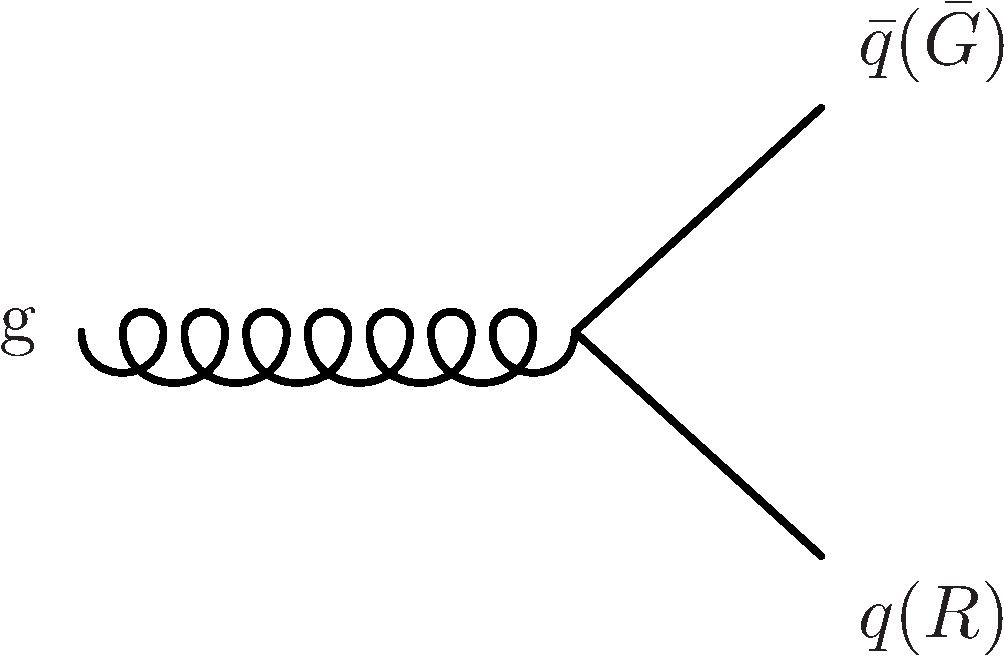
\includegraphics[width=0.7\textwidth]{./gluonVertex.pdf} 
\end{figure}
\end{minipage} \hfill
\begin{minipage}{0.45\textwidth}
An example we have seen before
\be
g\rightarrow q \bar{q}
\ee
q's have to have same mass, but can have different charge
\end{minipage}

\clearpage

Six quarks known to exist. 

\be
 \begin{pmatrix} u \\ d \end{pmatrix} \hspace*{0.1in}   \begin{pmatrix} c \\ s \end{pmatrix} \hspace*{0.1in}   \begin{pmatrix} t \\ b \end{pmatrix}  \hspace*{0.2in} \begin{matrix} +\frac{2}{3} \\ -\frac{1}{3} \end{matrix}
\ee
Have seen explicit evidence for  all six.

\be
 \begin{pmatrix} m_u  = 0.3\ \rmt{GeV}\\ 0.3 \end{pmatrix} \hspace*{0.1in}   \begin{pmatrix} 1.5 \\ 0.5 \end{pmatrix} \hspace*{0.1in}   \begin{pmatrix} 175 \\ 5 \end{pmatrix} 
\ee
All inferred from bound states or from  decays products.


No evidence for the existence of free quarks despite great efforts to find them. 

Have looked in 
\bi
\item[-] Moon rocks
\item[-] oyster shells
\item[-] deep sea sludge
\item[-] cosmic rays
\item[-] accelerators
\ei

However, over 200 quark bound states have been found.

\underline{Baryons} made of three quarks or anti-quarks  \multiline{$qqq$ \\ $\bar{q}\bar{q}\bar{q}$}

\bc
\textbf{examples:}  p, n, $\Lambda$, ect  (1/2 integer spins)
\ec

\underline{Mesons} made of  quarks/ anti-quarks pair  $q\bar{q}$

\bc
\textbf{examples:}  $\underbrace{\pi}_{\substack{u\bar{u} \\ u\bar{d} \\ d\bar{u}}}$,  $\underbrace{K}_{\substack{sX \\ \bar{s}X}}$, $\underbrace{D}_{cX}$, $\underbrace{B}_{bX}$  (Integer Spins)
\ec

For the strong and EM interaction, $q$ and $\bar{q}$ are only created or destroyed in pairs. 
$\Rightarrow$ for these interactions, Quantum Number associated with each quark flavour and overall Baryon number

eg:
\bea
  p + p &\rightarrow& n  + p + \pi^+ \\ 
  (uud) + (uud) &\rightarrow& (udd) + (uud) + (u\bar{d}) 
\eea

However not true for weak interactions 

eg: $\beta$ decay

\bea
  n  &\rightarrow&  p + e^- + \bar{\nu}_e \\ 
  (udd) &\rightarrow& (uud) + e^- + \bar{\nu}_e 
\eea

\begin{minipage}{0.6\textwidth}
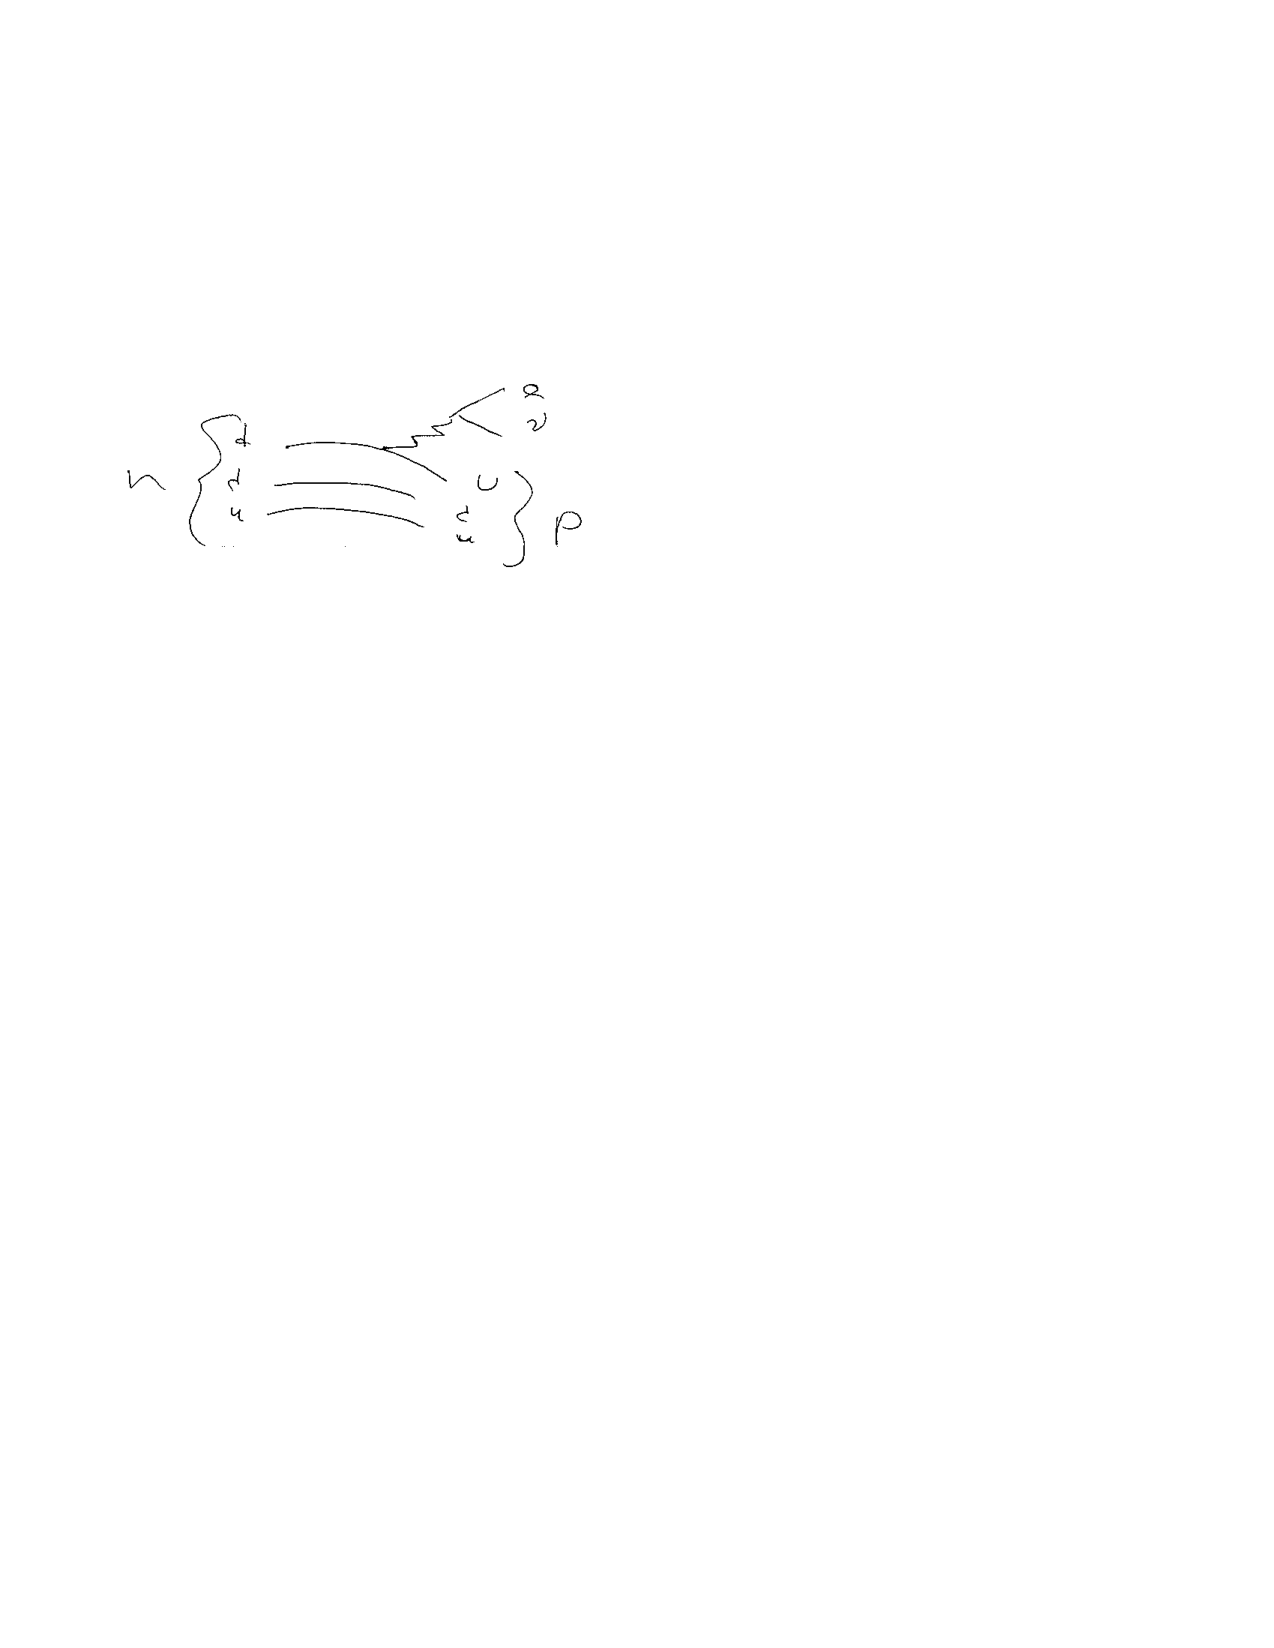
\includegraphics[width=0.8\textwidth]{./NeutronDecay.pdf}
\end{minipage} \hfill
\begin{minipage}{0.45\textwidth}
$N_d^i \ne N_d^f$
indication of the weak interaction
\end{minipage}


\underline{Pions}

\bc
 $\pi^\pm$ (m = 0.140) decays  $\pi^\pm \rightarrow \mu^\pm + \nu_\mu$ with lifetime $10^{-5}$s \\ 
 $\pi^0$  (m = 0.135) decays  $\pi^0 \rightarrow \gamma\gamma$ with lifetime $10^{-16}$s \\ 
\ec

As for leptons, Quantum numbers associated with flavours of quarks. 

eg: strange-ness (s) or charm-ness (c) 

Again, these are not conserved in weak interactions 

\underline{Lifetimes of Particles} Critical for understanding underlying symmetries/dynamics 

(Also easy to measure) 

\bi
\item[-] typical timescale associated to strong interactions $\sim r_{\rmt{nucleus}} \sim 10^{-23}s$
\item[-] typical timescale associated to electromagnetic interaction $\sim 10^{-16} - 10^{-21}$s
\item[-] typical timescale associated to weak interaction $\sim 10^{-7} - 10^{-13}$ s
\ei

\clearpage

\underline{``Strange Particles''}

Particles produced via strong interactions by decay via the weak interaction $\rightarrow$ long life-times.

$\Rightarrow$ existence of new quantum number. 

\bea
\Lambda &\rightarrow& \pi^- + p (65\%)\\
        &\rightarrow& \pi^0 + n (35\%)
\eea

\be
\underbrace{uds}_{S=-1} \rightarrow \underbrace{d\bar{u} + uud}_{S = 0}
\ee

$\Lambda$ - lightest strange Baryon \\
$K$ - lightest strange Meson

Can be produced strongly via associated production 
eg:

\be
\underbrace{\pi^- + p}_{S=0} \rightarrow \underbrace{K + \Lambda}_{S = 1  -1}
\ee

Discovery of strange particles caused great excitement in the field because they represented a new form of matter completely \underline{unexpected}.

In 1974, the discovery of charmed particles caused equally great excitement because their existence was expected. 

This was decisive in determining the correctness of the ``electro-weak'' theory and the quark model.   

}
\end{document}

